\section{An Introduction to the application}
Hello and welcome to the user guide for MuseLib. This is an application which takes a collection of sheet music files and automatically collects data about each piece, and provides you with an organiser displaying them in different categories.
\section{Files you can use}
This application can only get information about files which are of the MusicXML file type. If you have MuseScore, Sibelius, Finale or many other editors as your composition software of choice, then you can use this app! All you have to do is export the files you've created to the MusicXML format using the export options in your particular program. Once you've done that, put them all in one folder and we'll get started.

\section{Getting Started}
\begin{figure}[H]
\centering
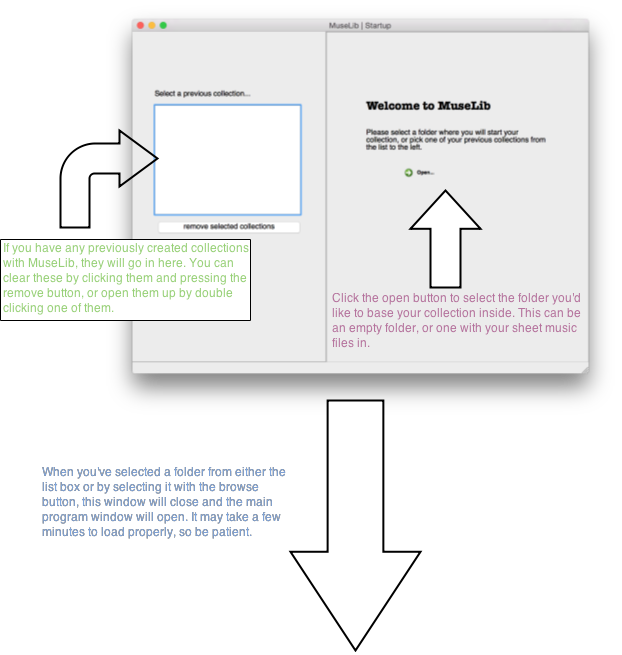
\includegraphics[width=\textwidth]{startup}	
\end{figure}

\subsection{Main window}
\begin{figure}[H]
\centering
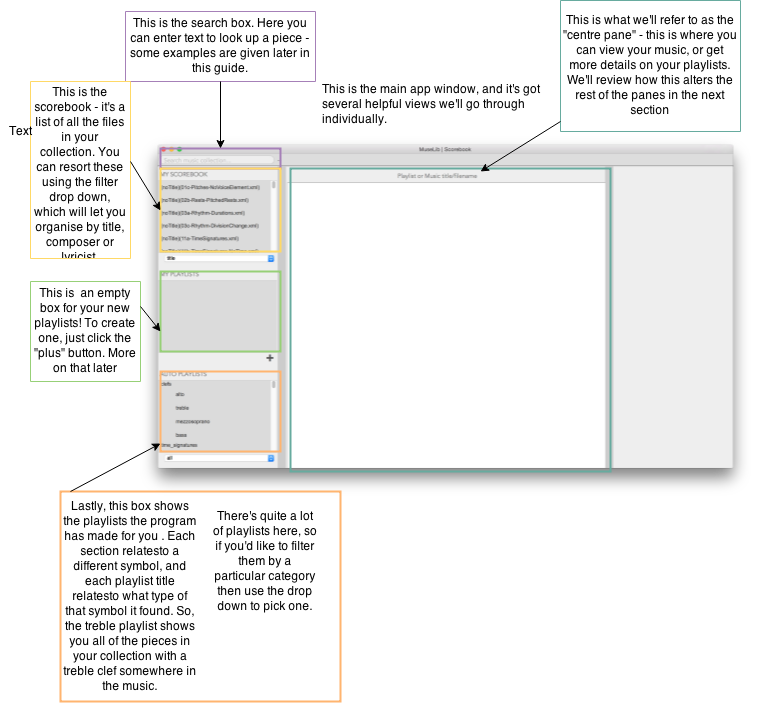
\includegraphics[width=500pt]{main_screenshot}	
\end{figure}

\subsection{Viewing Pieces}
\begin{figure}[H]
\centering
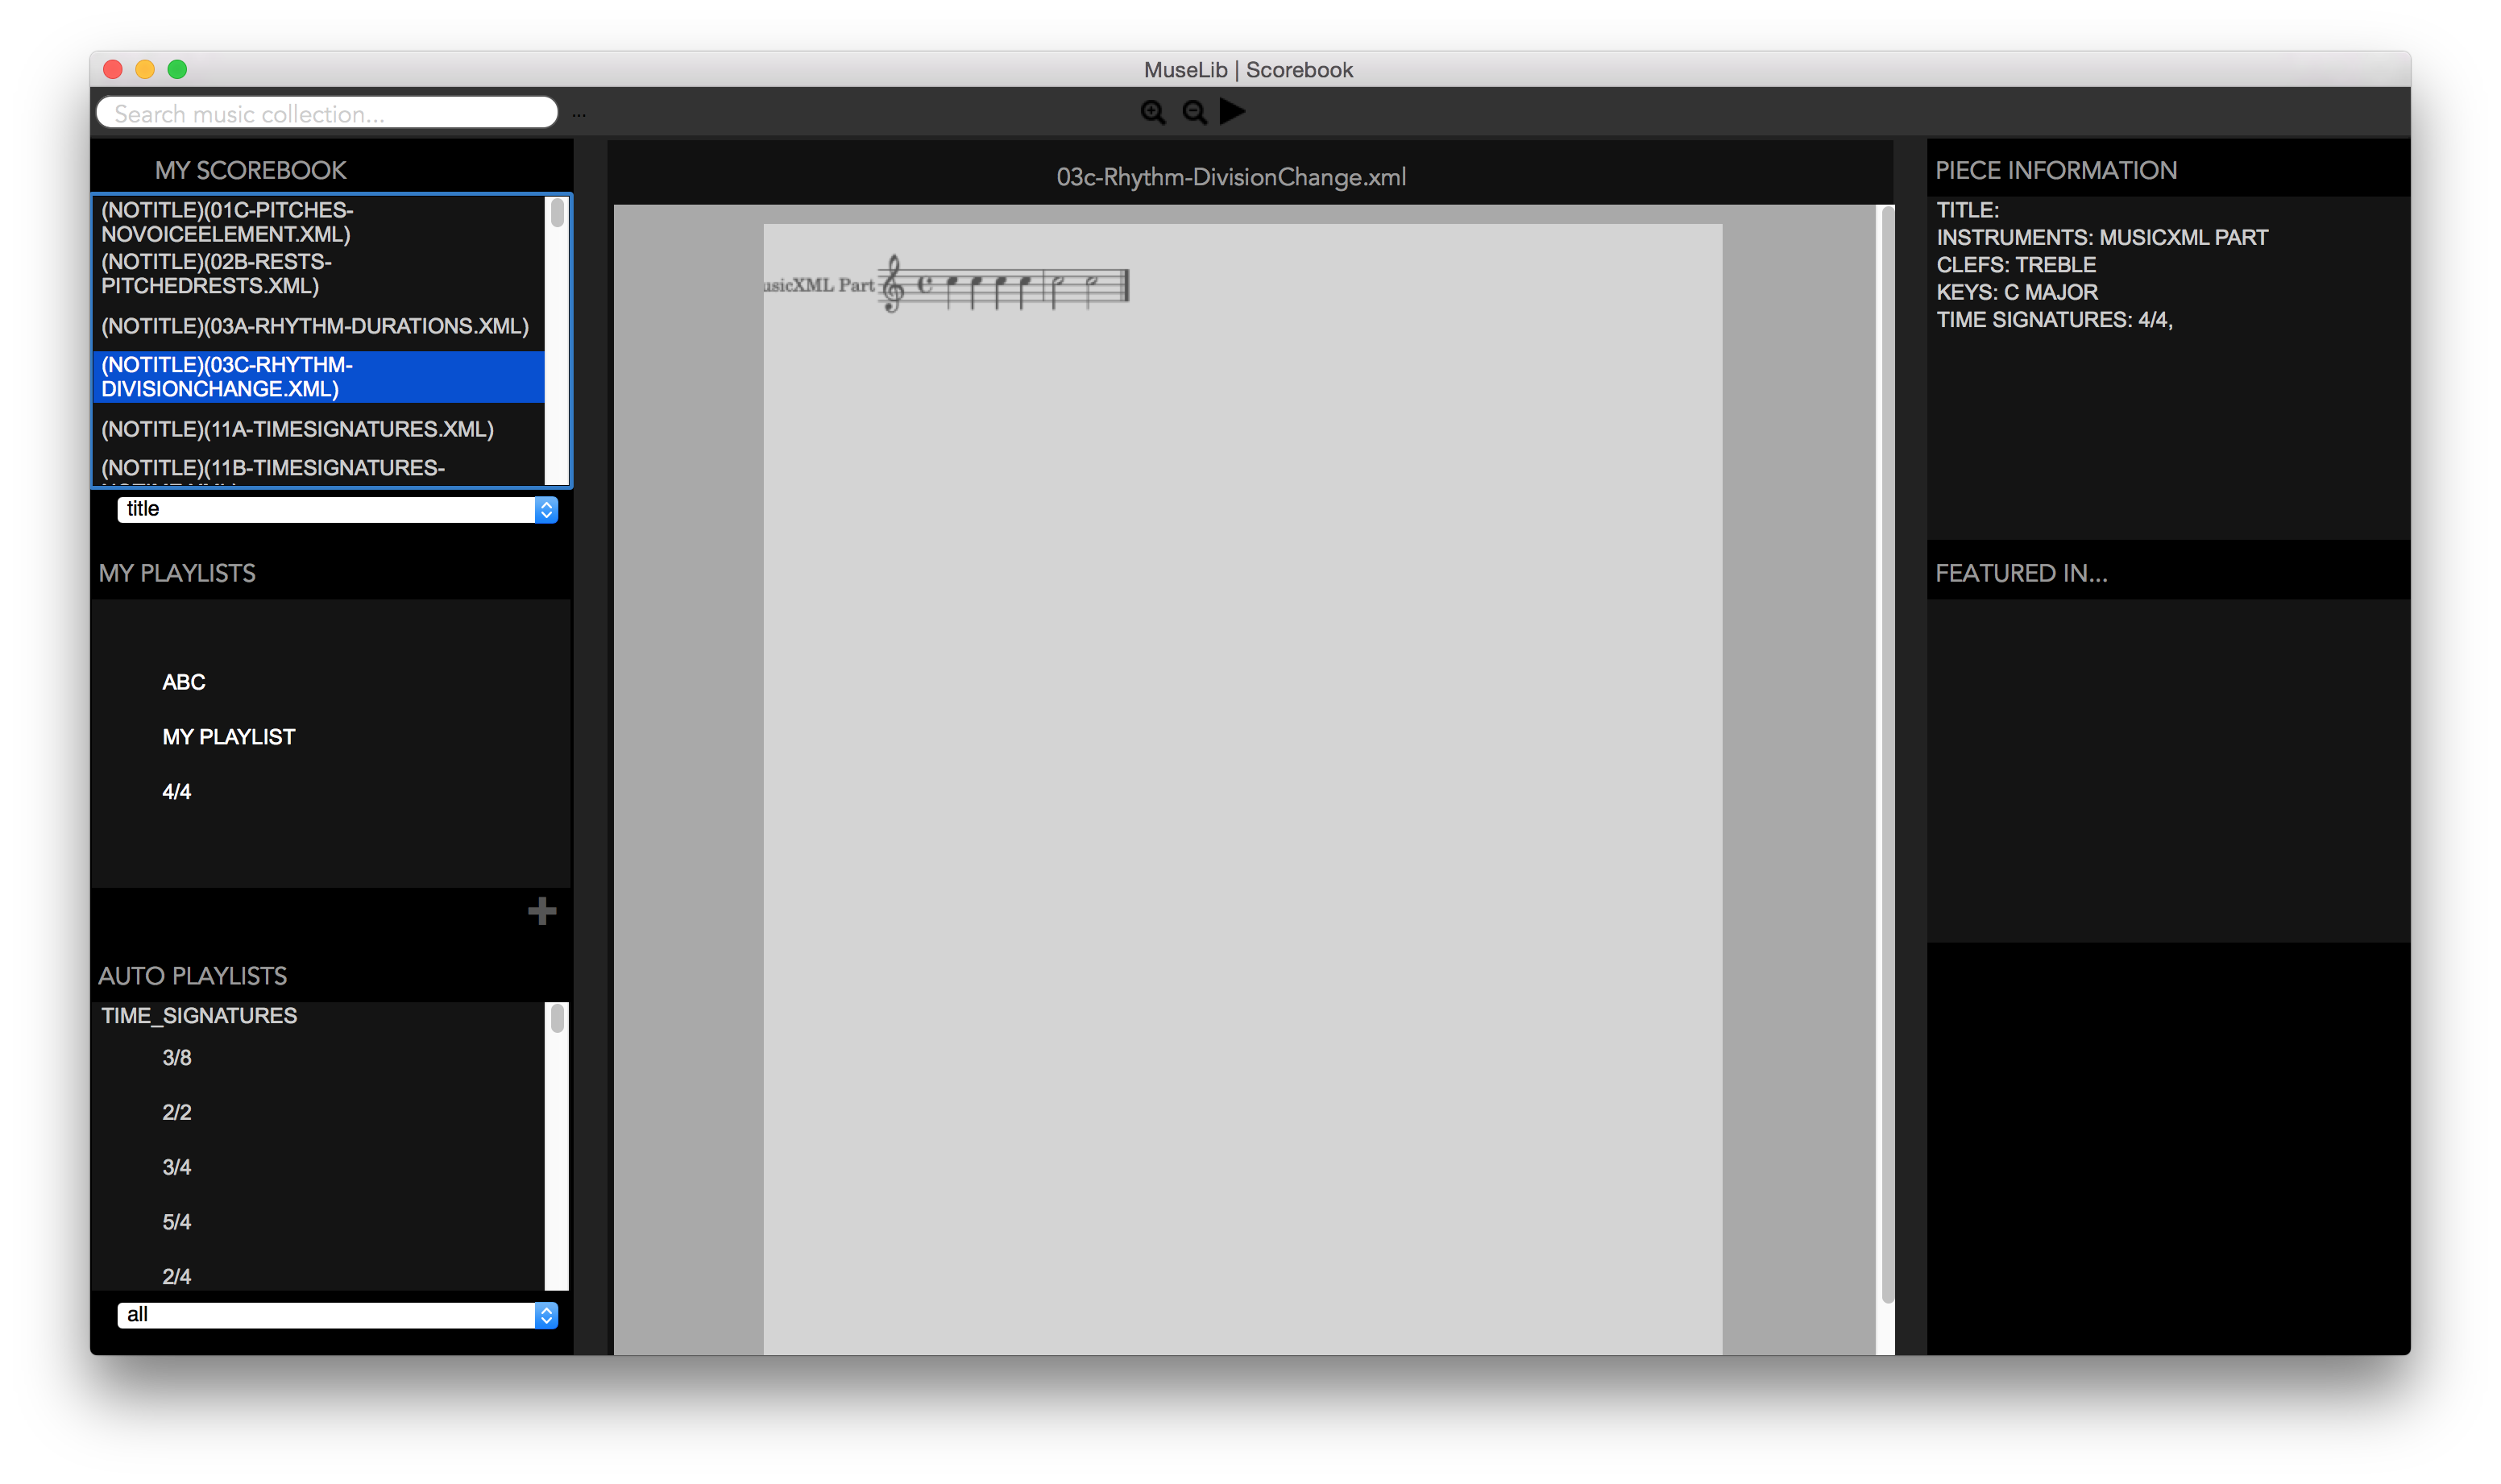
\includegraphics[width=500pt]{main_piece}	
\end{figure}

\section{Playlists}
\subsection{Adding Playlists}
\begin{figure}[H]
\centering
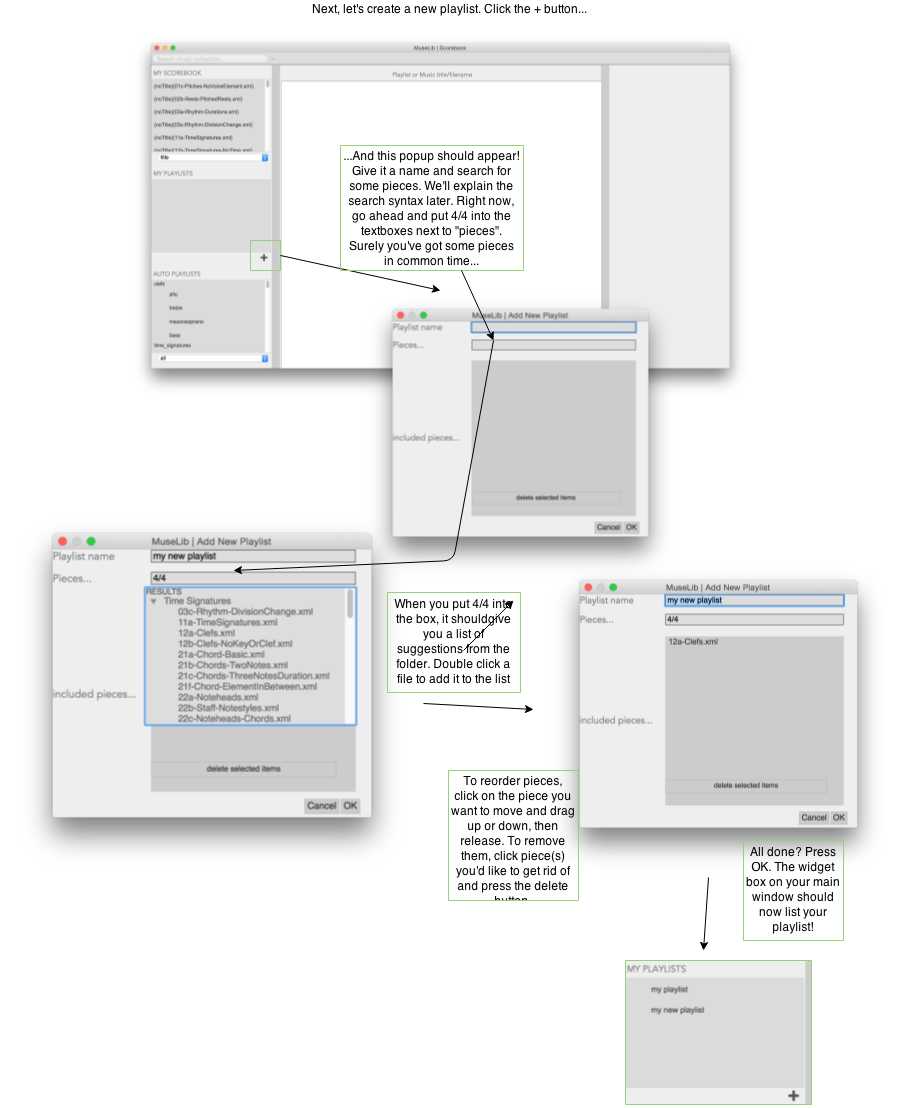
\includegraphics[width=500pt]{add-playlist}	
\end{figure}

\subsection{Viewing Playlists}
\begin{figure}[H]
\centering
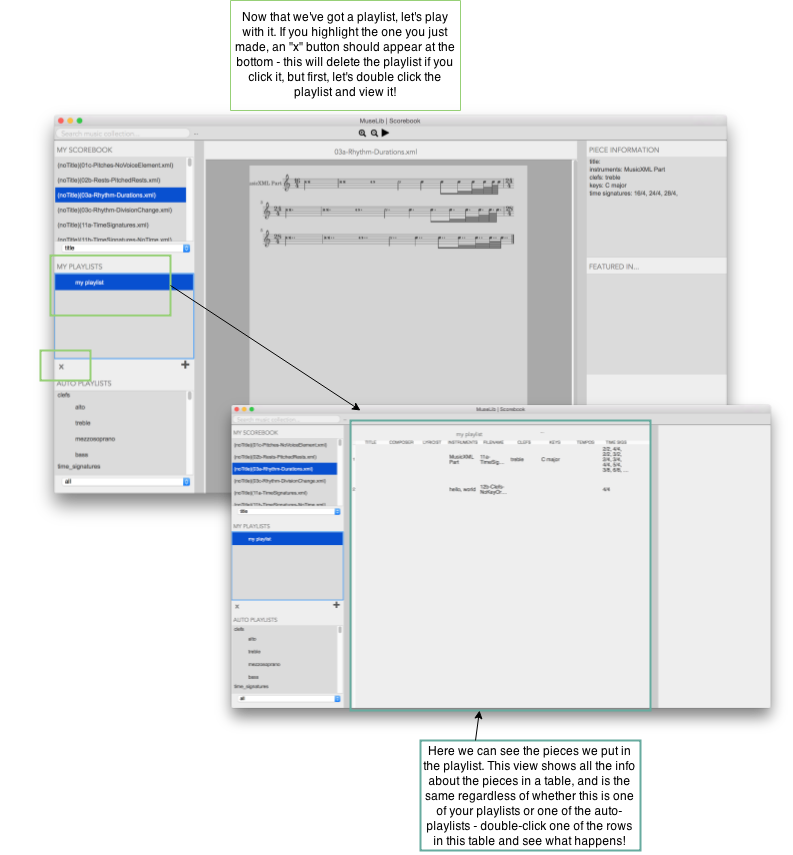
\includegraphics[width=500pt]{view-playlist}	
\end{figure}
\subsubsection{Viewing a Piece inside a Playlist}
\begin{figure}[H]
\centering
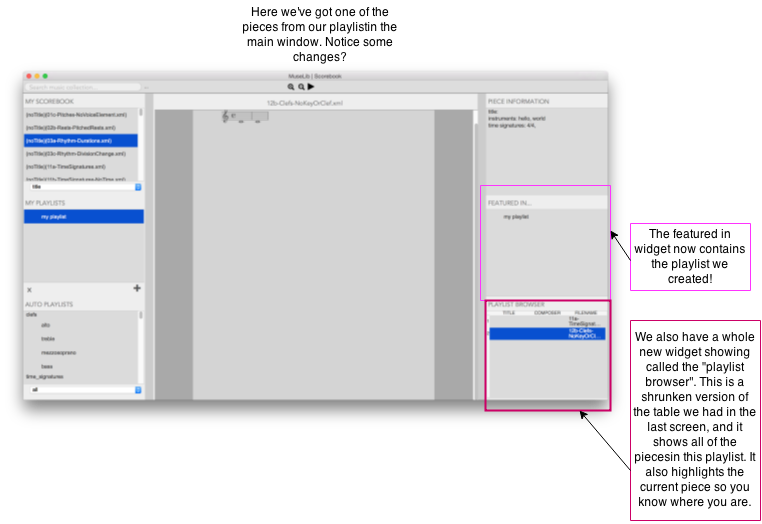
\includegraphics[width=500pt]{view-piece-playlist}	
\end{figure}
\section{Searching}
\subsection{Simple Searches}
\begin{figure}[H]
\centering
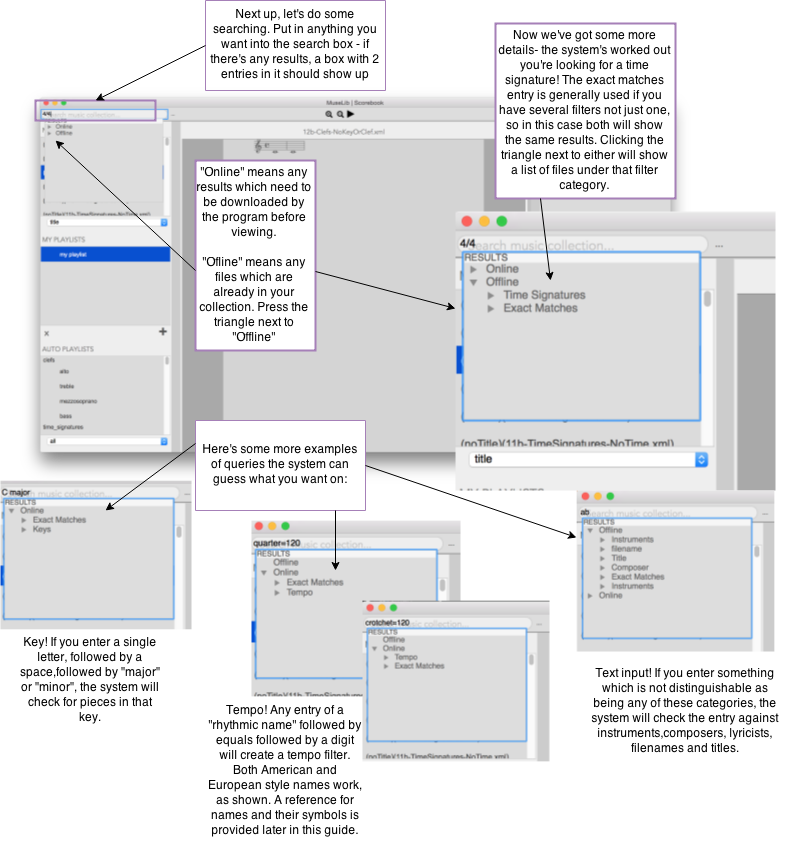
\includegraphics[width=500pt]{searching}
\end{figure}
\subsubsection{Rhythm names}
The above guide references rhythm names. These are the different names given to note symbols depending on their durations. The table below provides a general guide.


\subsection{Complex Searches}
\begin{figure}[H]
\centering
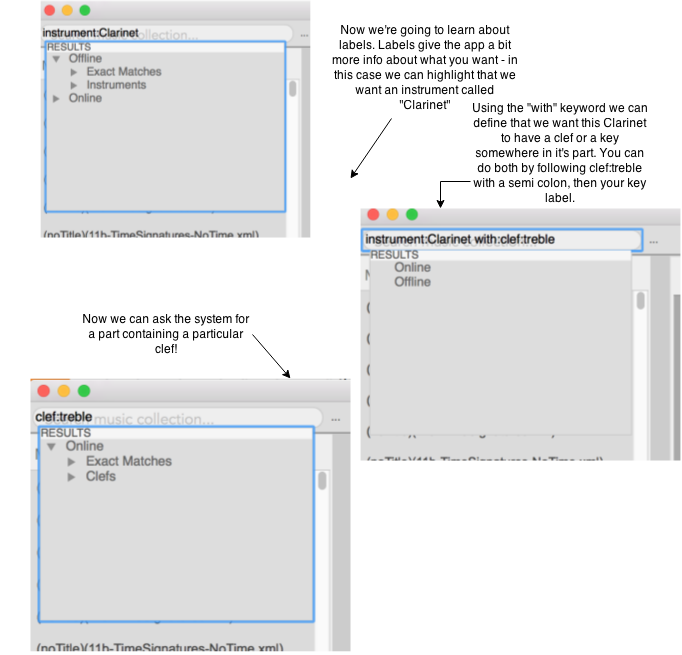
\includegraphics[width=500pt]{complex-searching}
\end{figure}
\subsubsection{Labels}
The guide in this section references "labels". The following table provides information on all the labels provided for searches.

\begin{table}[H]
\begin{tabu} to 1.05\textwidth {| X[l] | X[l] |} \hline
{\textbf{Command}} & {\textbf{Result}} \\ \hline
key:"C major" & System will look for pieces in this key \\ \hline
clef:treble & System will look for pieces with this clef in any part \\ \hline
tempo:quarter=120 & System will look for pieces with the tempo quarter note 120 quarter beats per minute. \\ \hline
meter:4/4 & System will search for a time signature \\ \hline
instrument:clarinet with:key:"C major" & System will search for pieces containing the instrument "clarinet" which is in the key of C major at some point in the piece \\ \hline
instrument:clarinet with:clef:bass & System will search for pieces containing the clarinet where the clarinet has a bass clef somewhere in the piece \\ \hline
instrument:clarinet with:clef:bass;key:"C major" & System will search for pieces containing the clarinet where the clarinet has a bass clef somewhere in the piece and is in C major somewhere in the piece \\ \hline
transposition:clarinet with:clef:bass;key:"C major" & System will search for pieces containing the clarinet, or if there is no clarinet, any instrument which has the same transposition \\ \hline
\end{tabu}
\caption{A table describing the command options for complex searches}
\label{table:commands_complex}
\end{table}

\subsection{Downloading Files}
\begin{figure}[H]
\centering
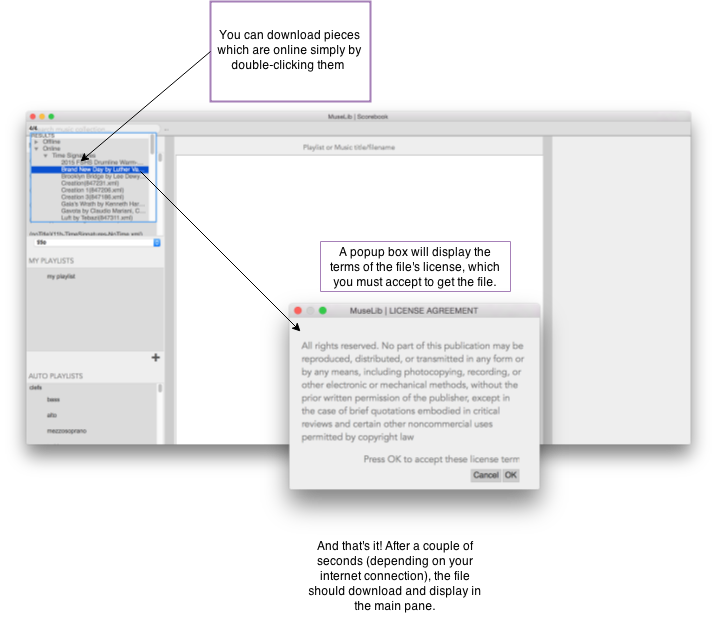
\includegraphics[width=500pt]{downloading}
\end{figure}


\section{Adding new files}
\begin{figure}[H]
\centering
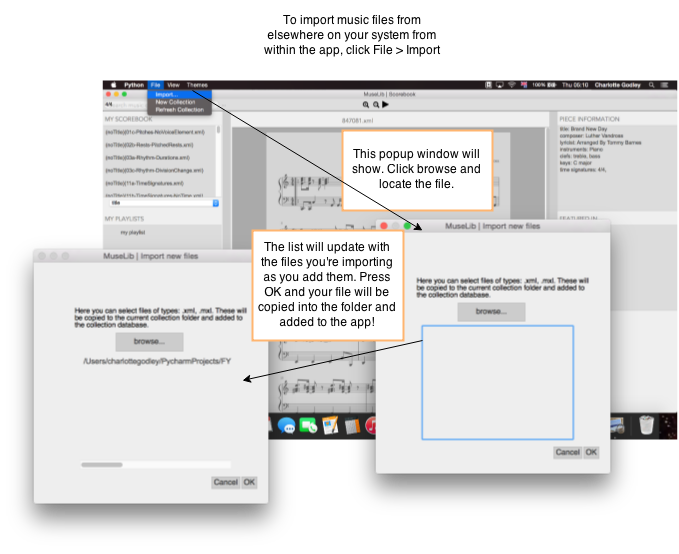
\includegraphics[width=500pt]{import_files}
\end{figure}

\section{Error Popup}
Occasionally, files produce problems the system cannot handle - this includes drum tab and guitar tab. At other times there will be problems in the process the application could not process for different reasons, such as downloading files without internet connection. When these occur, the popup in figure \ref{fig:error} will display. If you find any odd errors, please report these to a developer.
\begin{figure}[H]
\centering
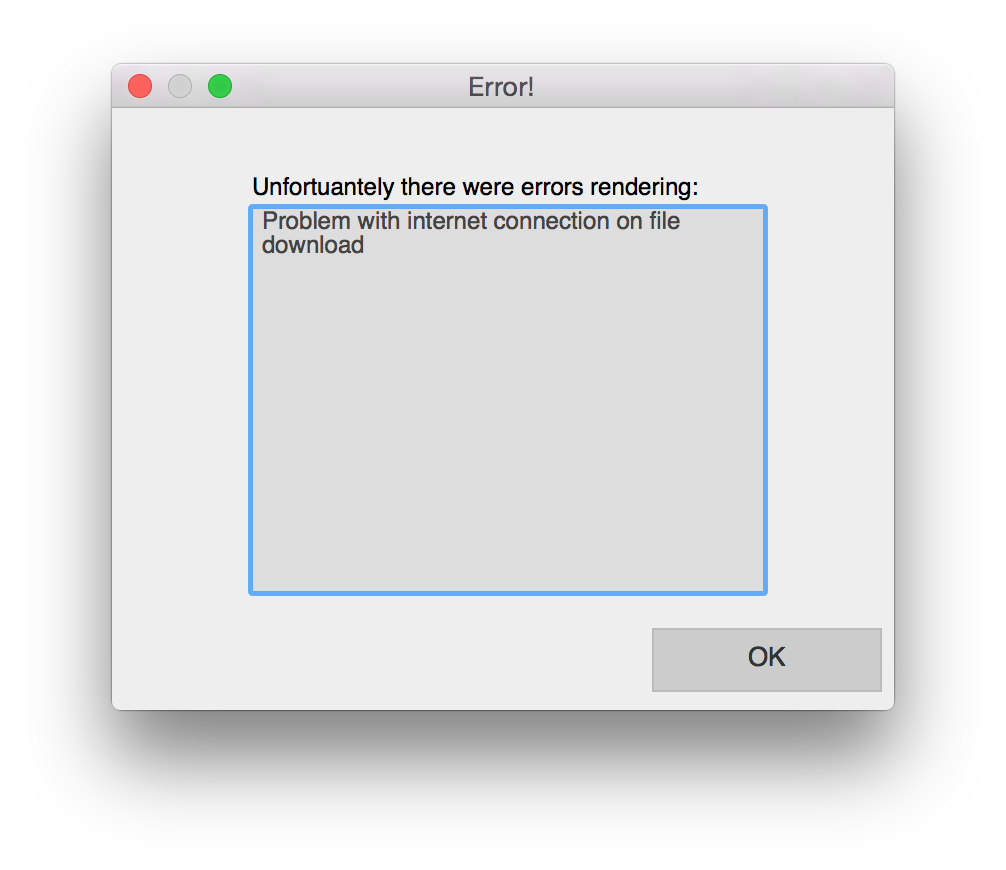
\includegraphics[width=500pt]{errorpop}
\caption{The window which will display on startup}
\label{fig:error}	
\end{figure}

\section{Customising your display}
\subsection{Themes}
The system comes with three different themes - the default which is light, dark and electric blue. These can be changed by clicking them in the theme menu as shown in figure \ref{fig:themes}. Their respective screenshots are shown in figures \ref{fig:theme2}, \ref{fig:theme3} and \ref{fig:theme4}.
\begin{figure}[H]
\centering
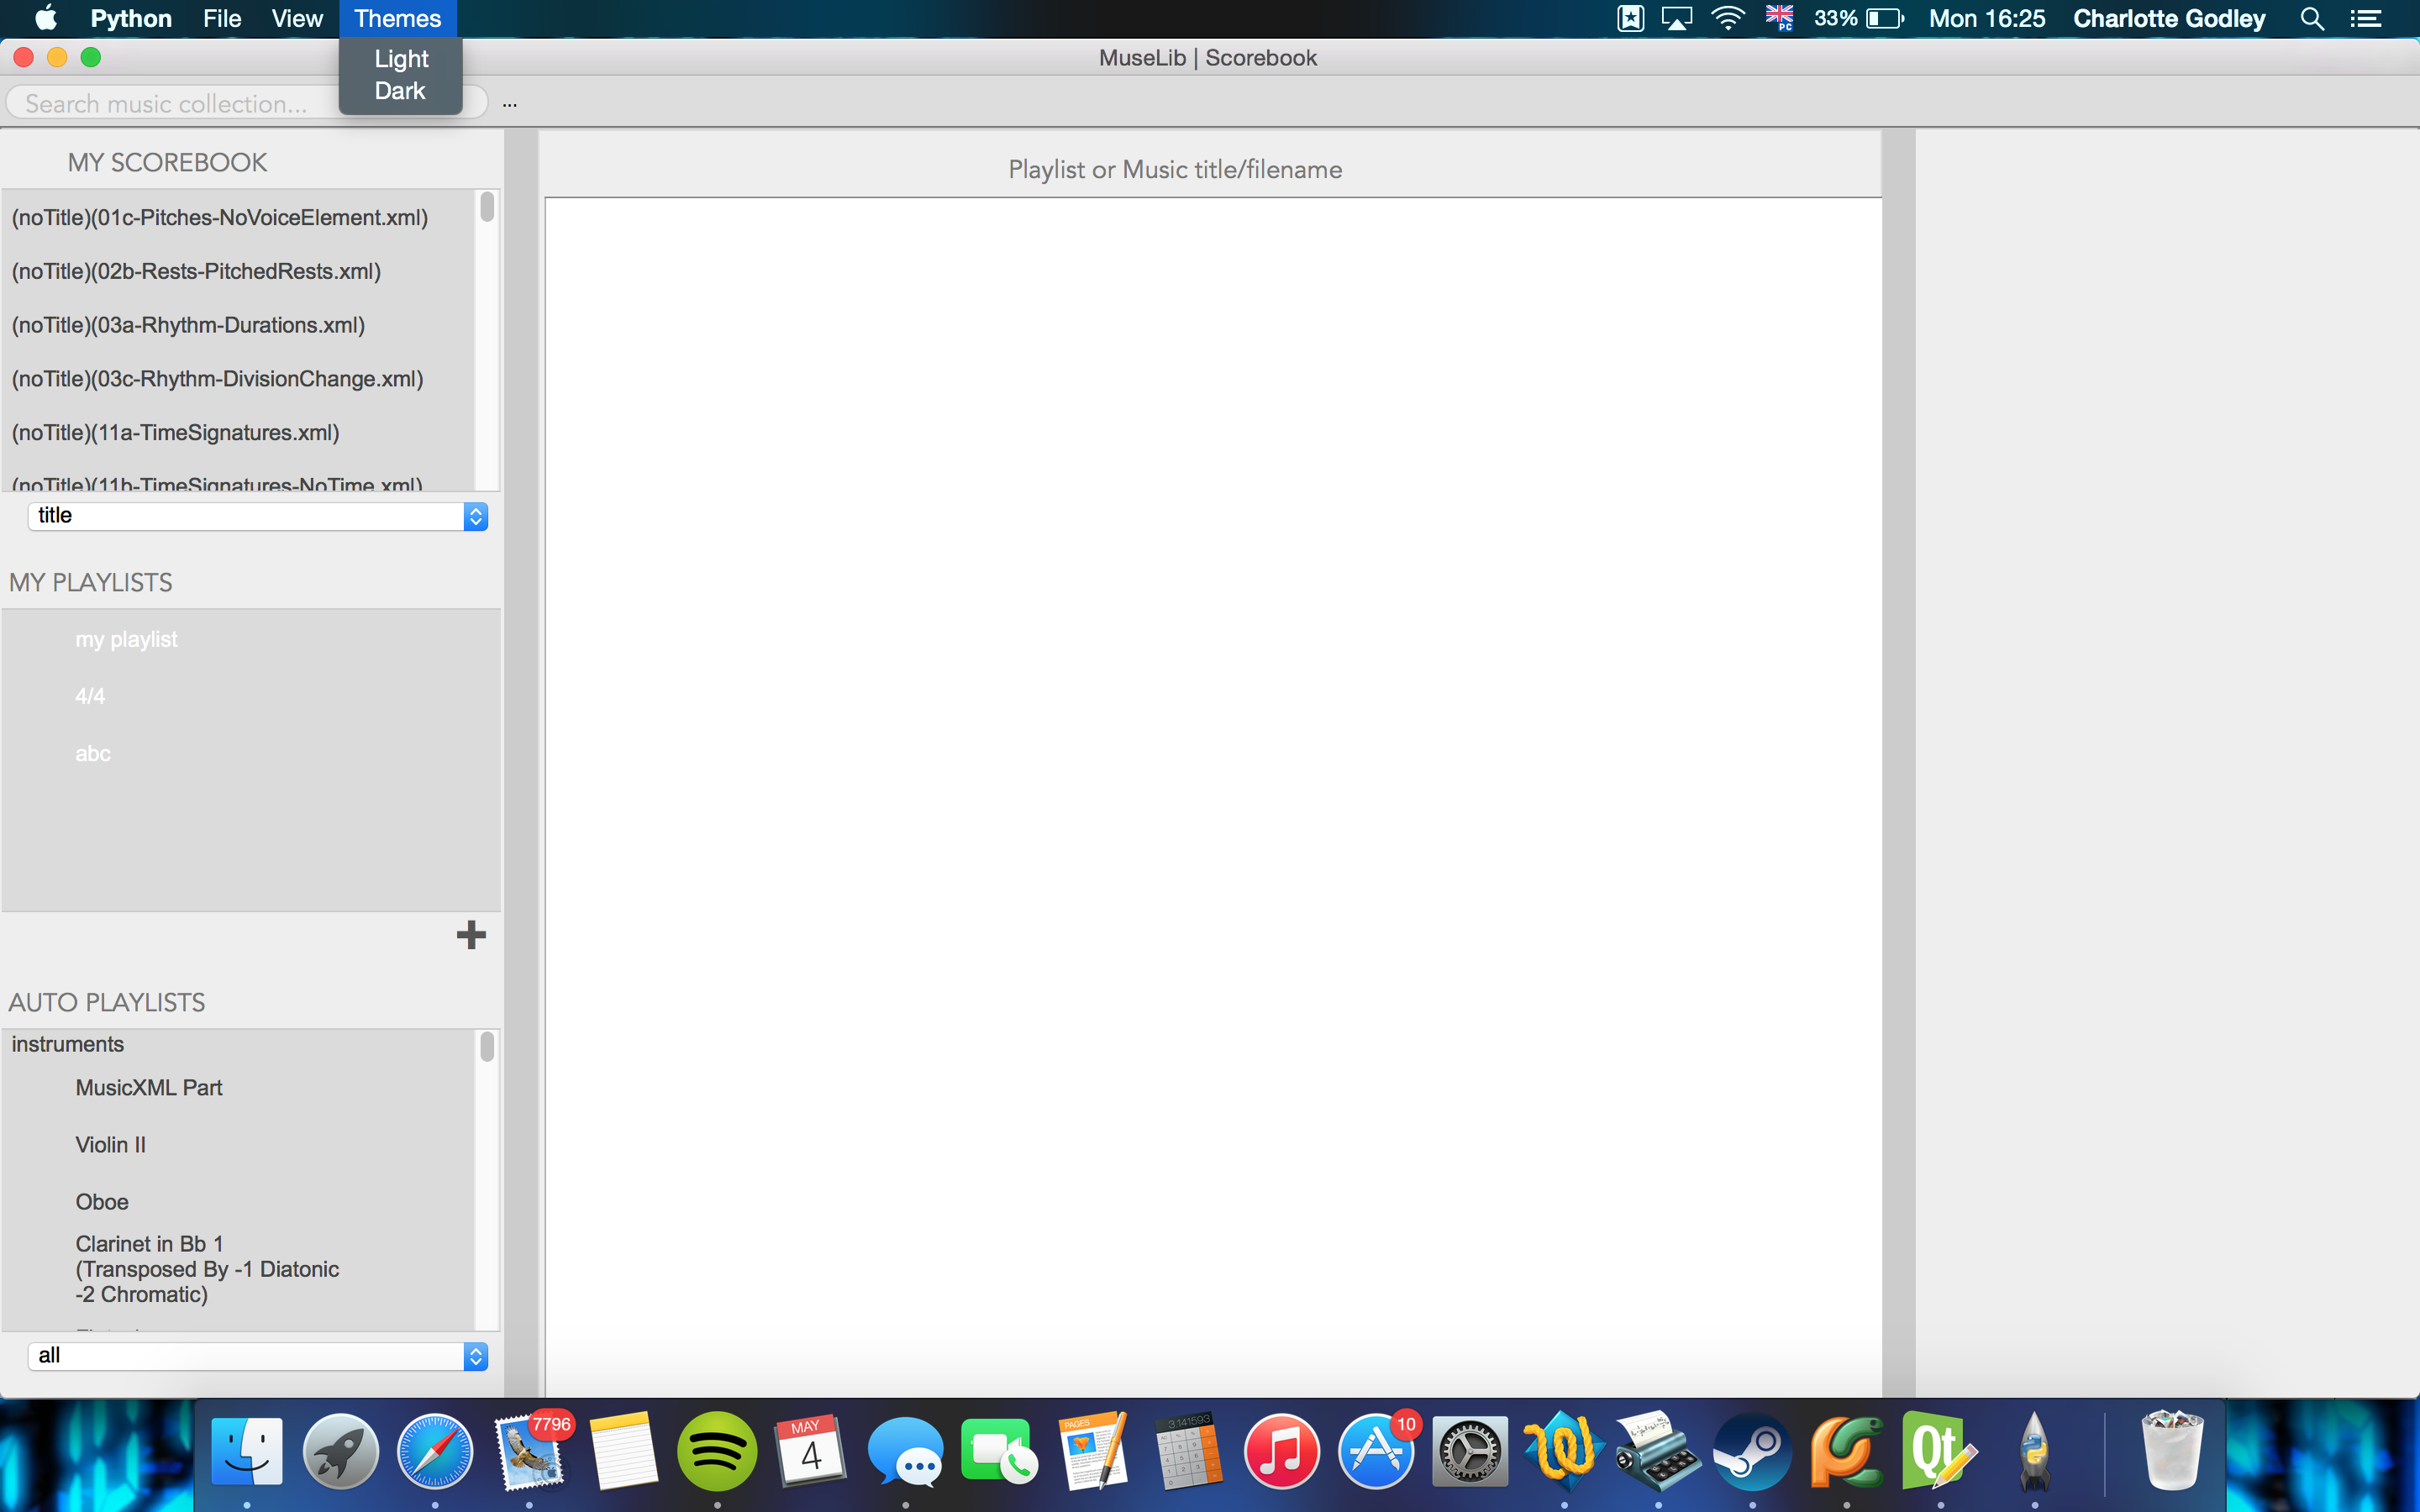
\includegraphics[width=500pt]{theme}
\caption{The themes menu}
\label{fig:themes}	
\end{figure}


\begin{figure}[H]
\centering
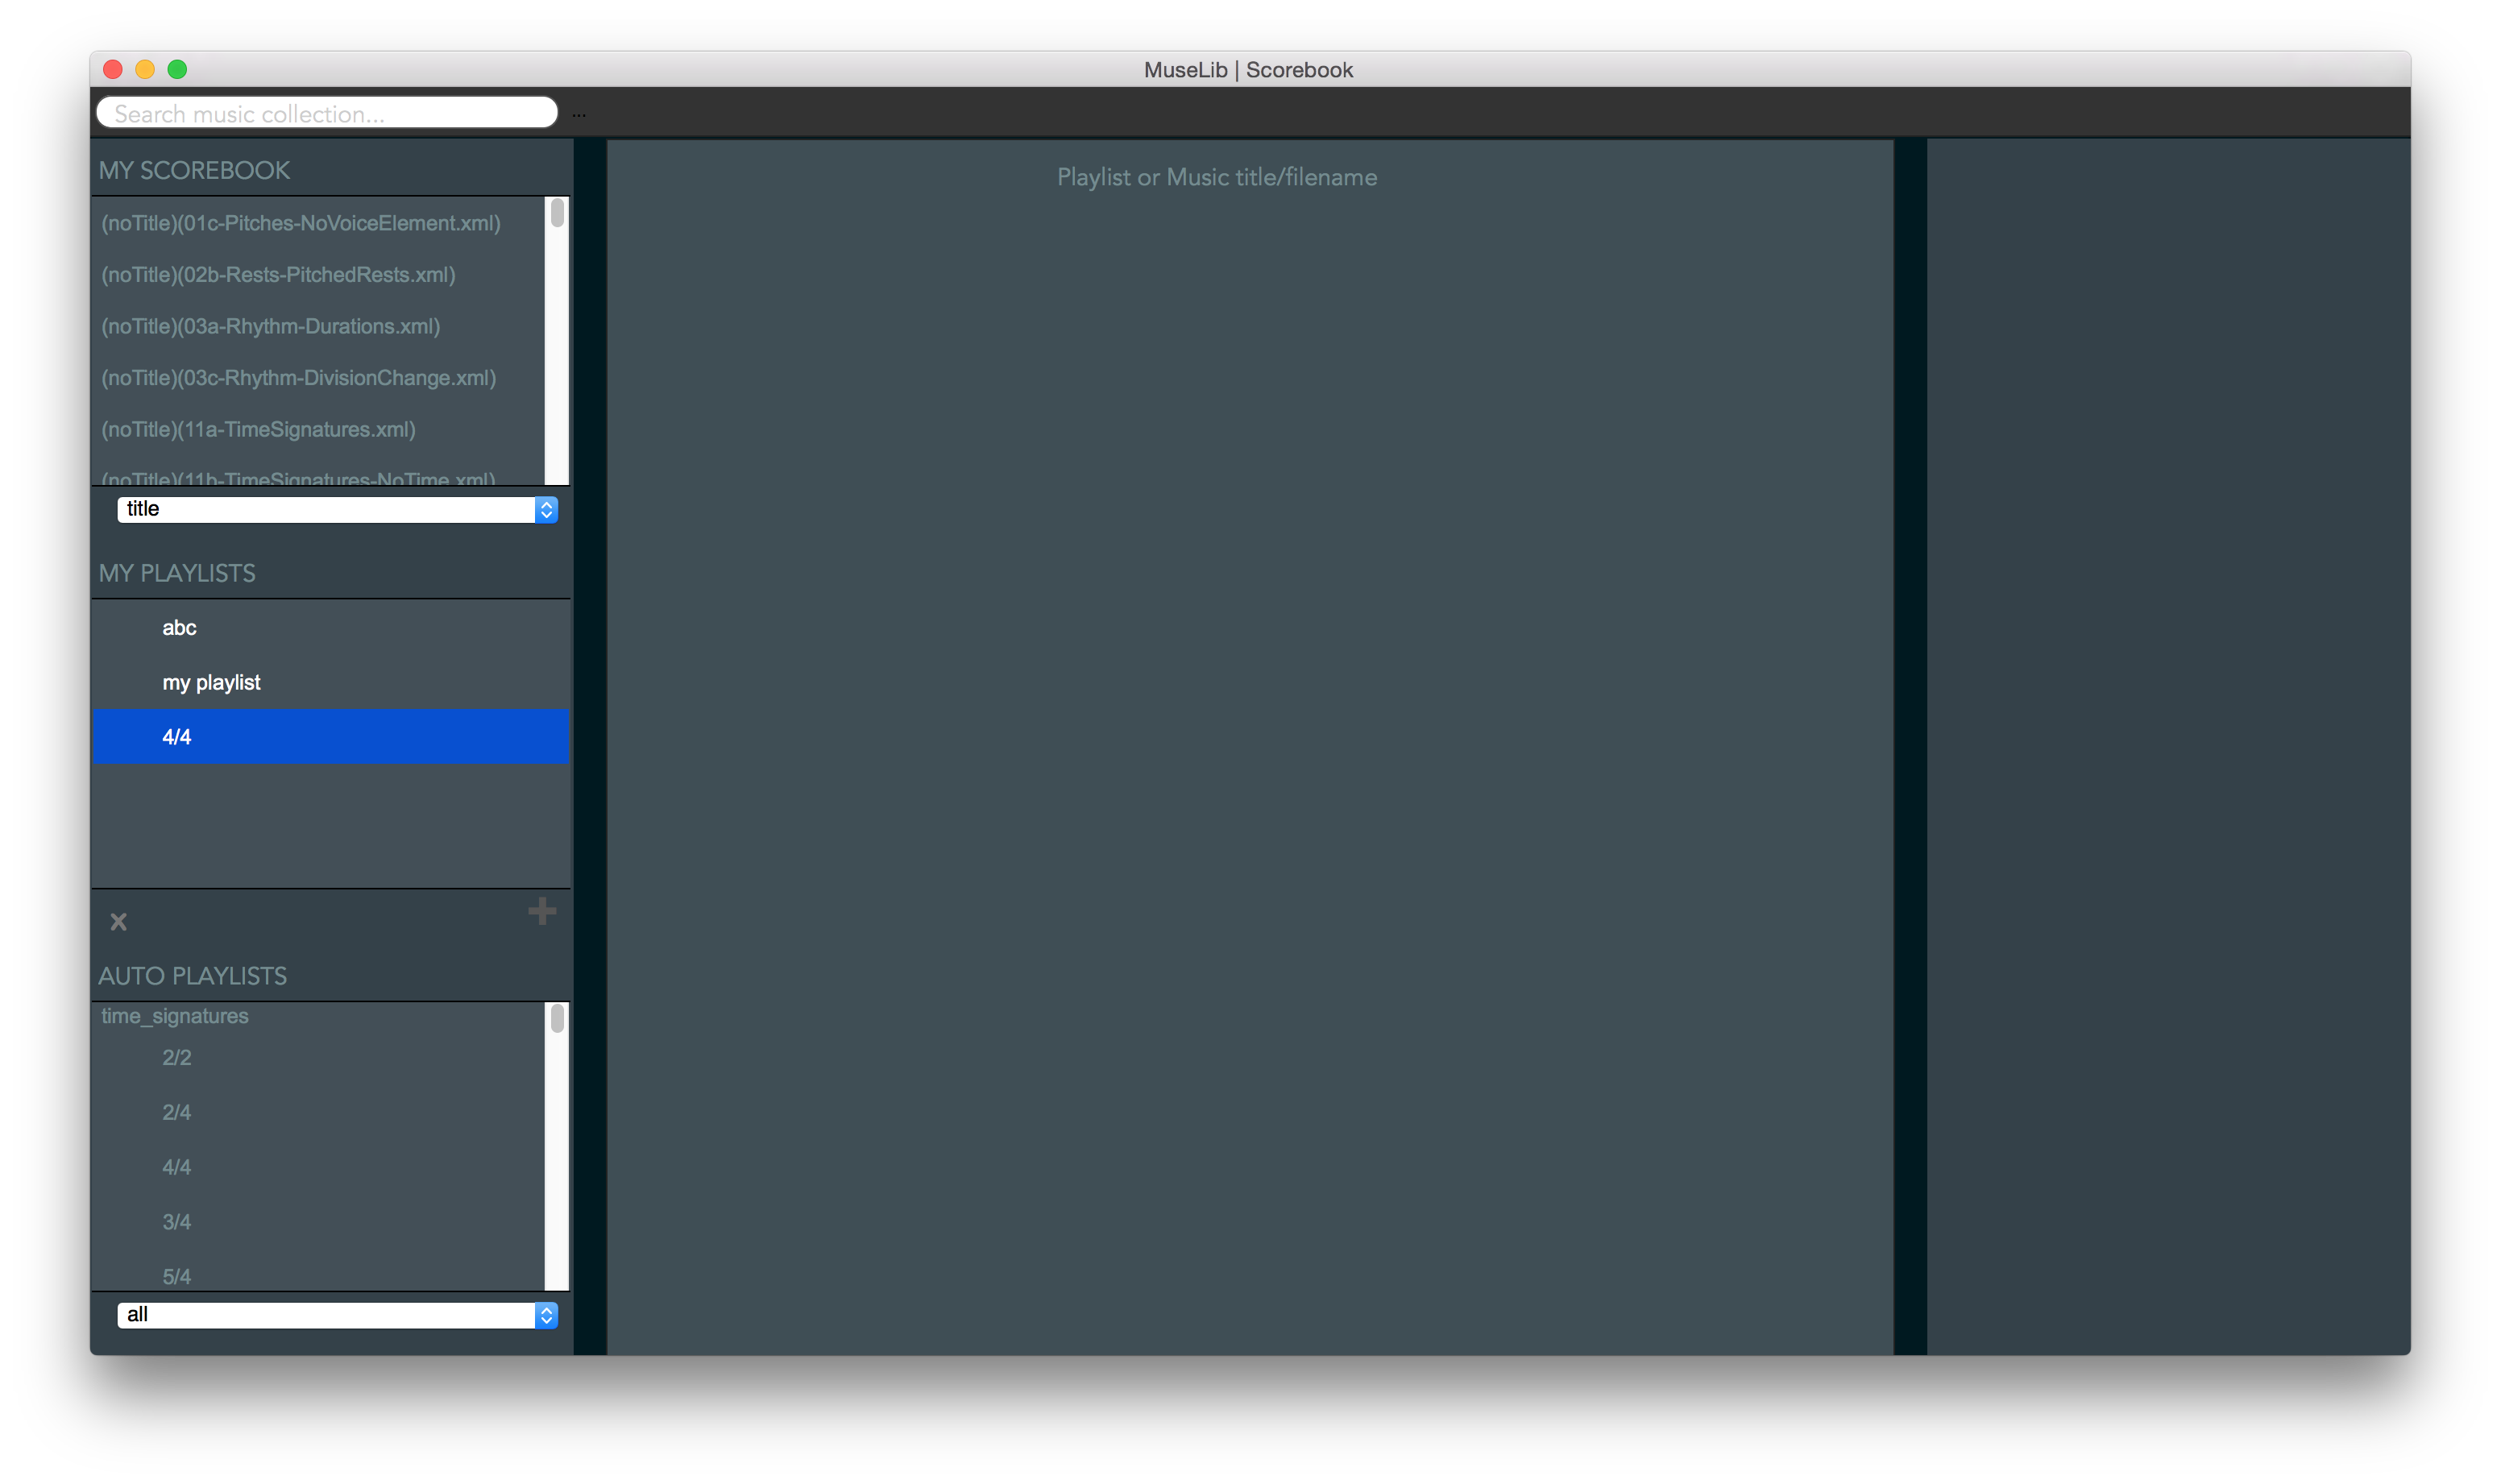
\includegraphics[width=400pt]{main_dark}
\caption{The dark theme}
\label{fig:theme2}	
\end{figure}

\begin{figure}[H]
\centering
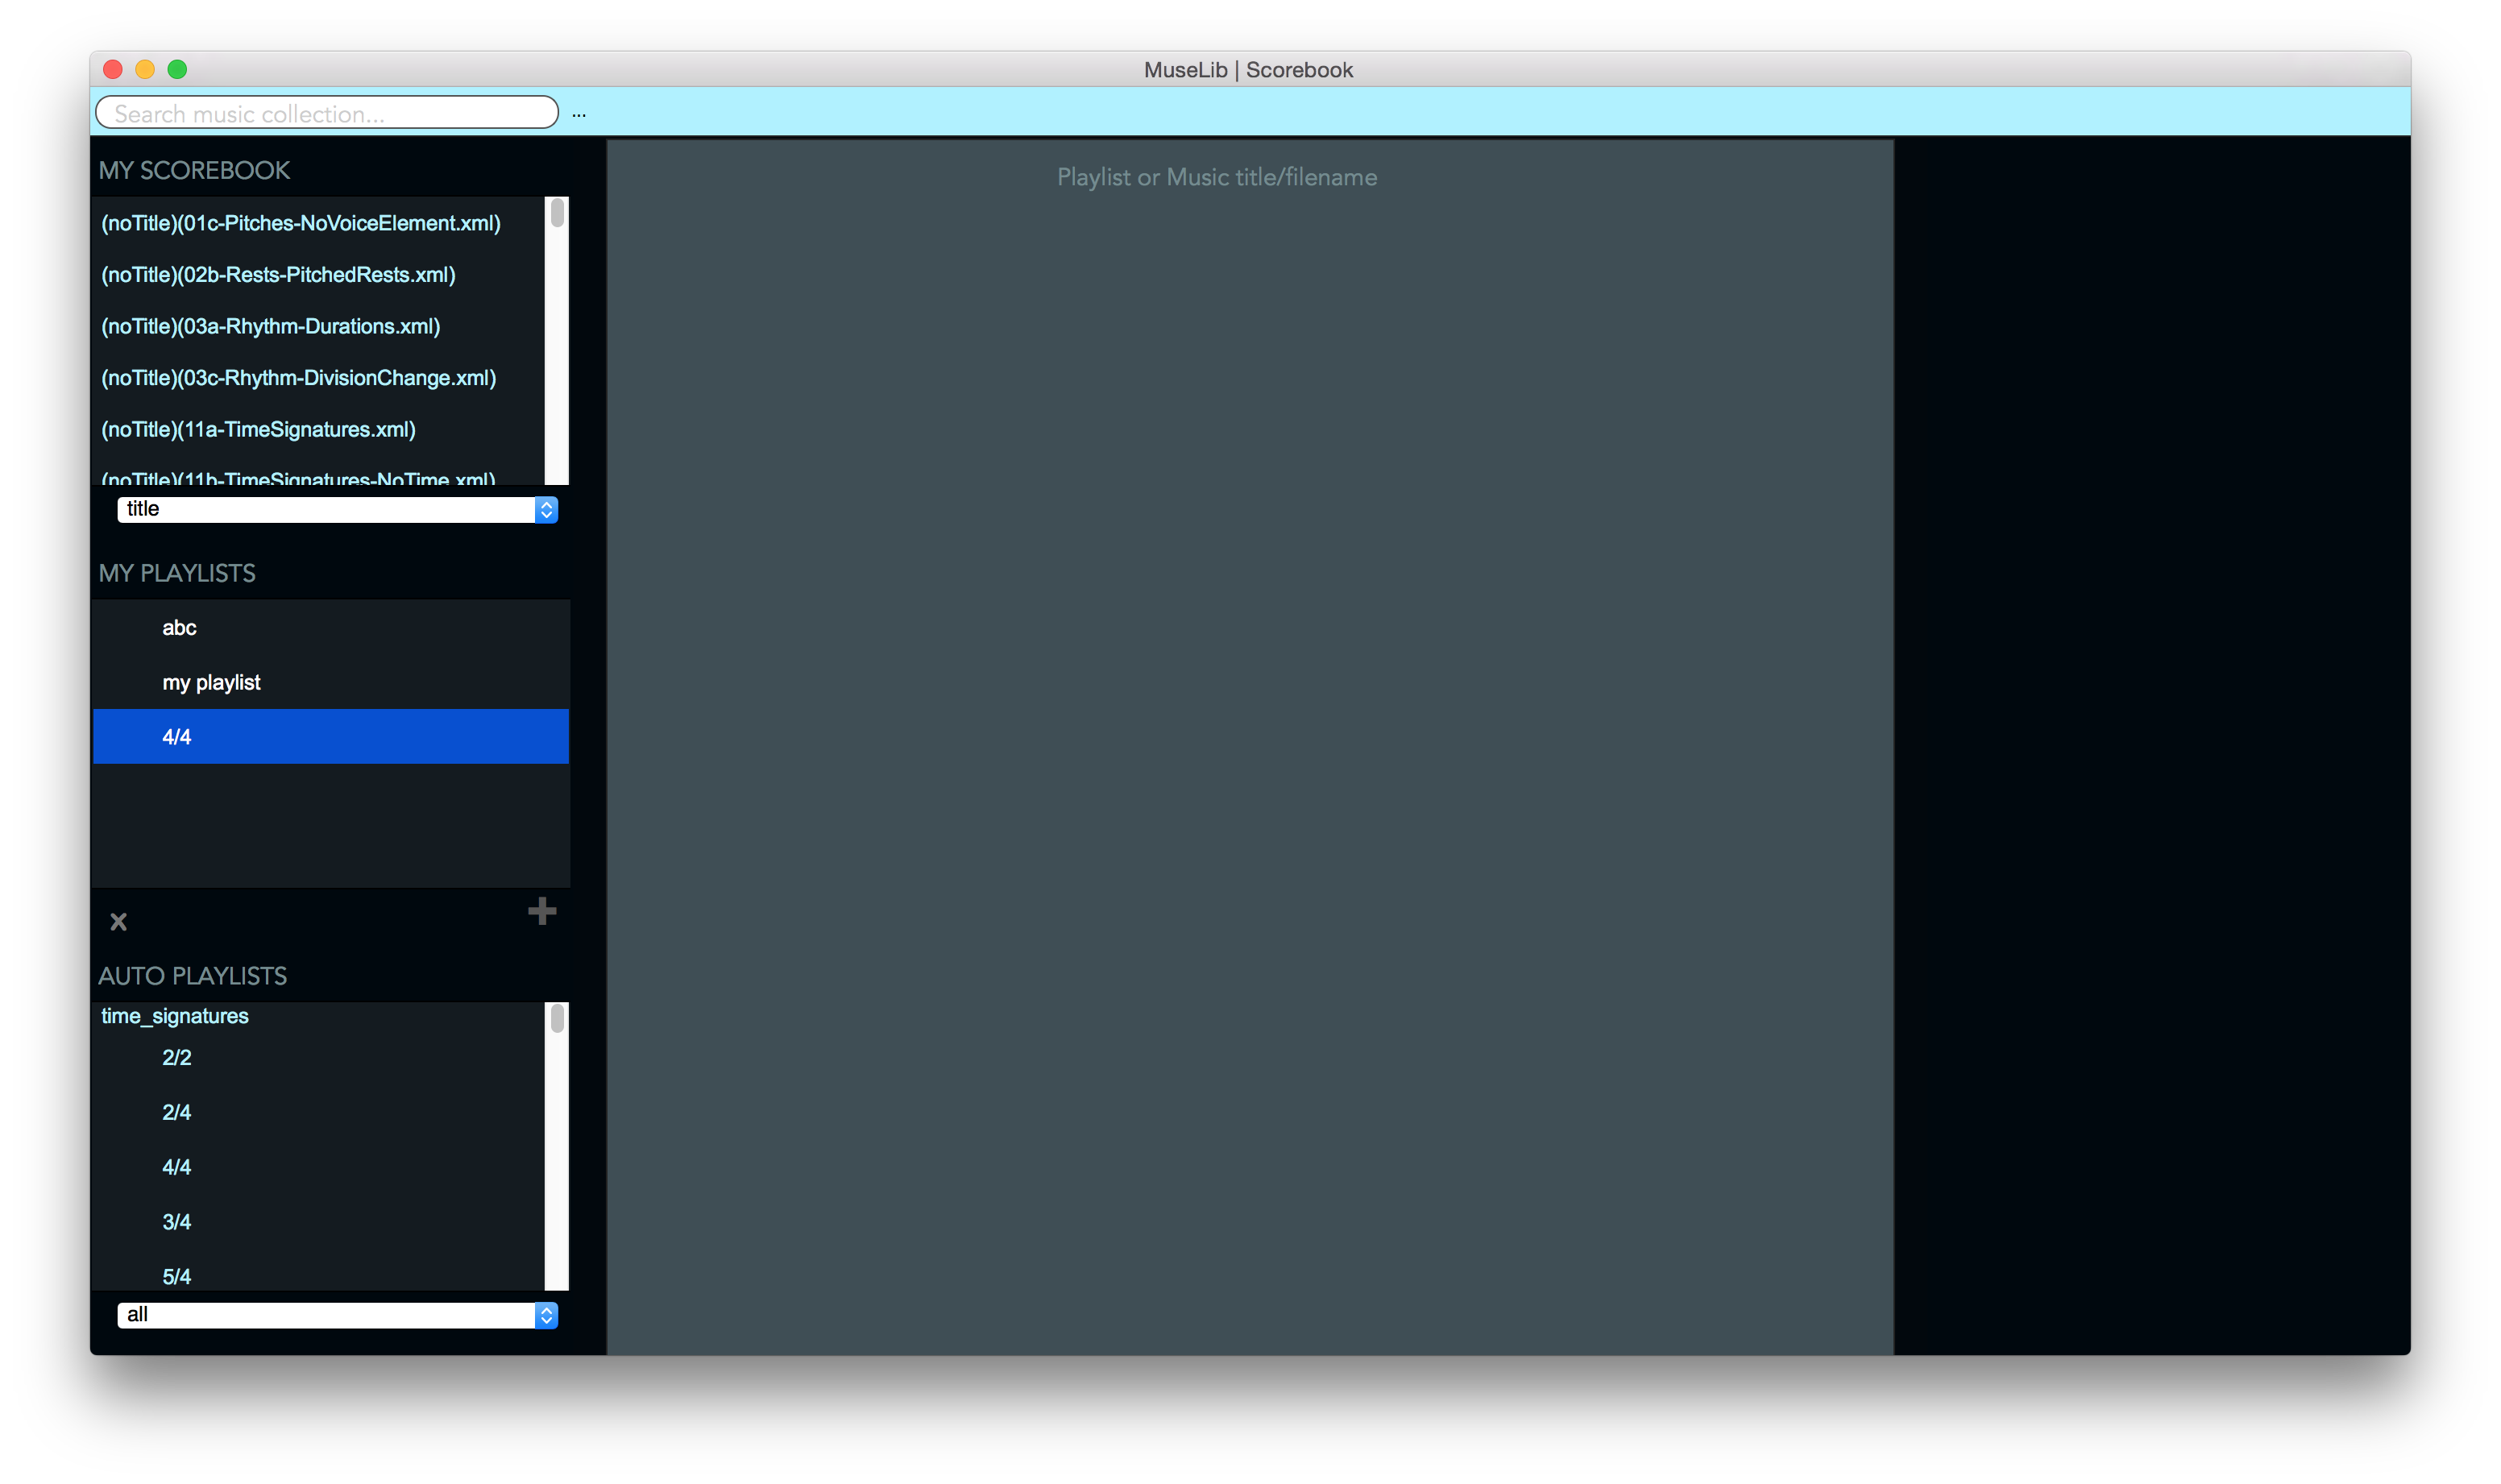
\includegraphics[width=400pt]{main_electric}
\caption{The electric blue theme}
\label{fig:theme3}	
\end{figure}

\begin{figure}[H]
\centering
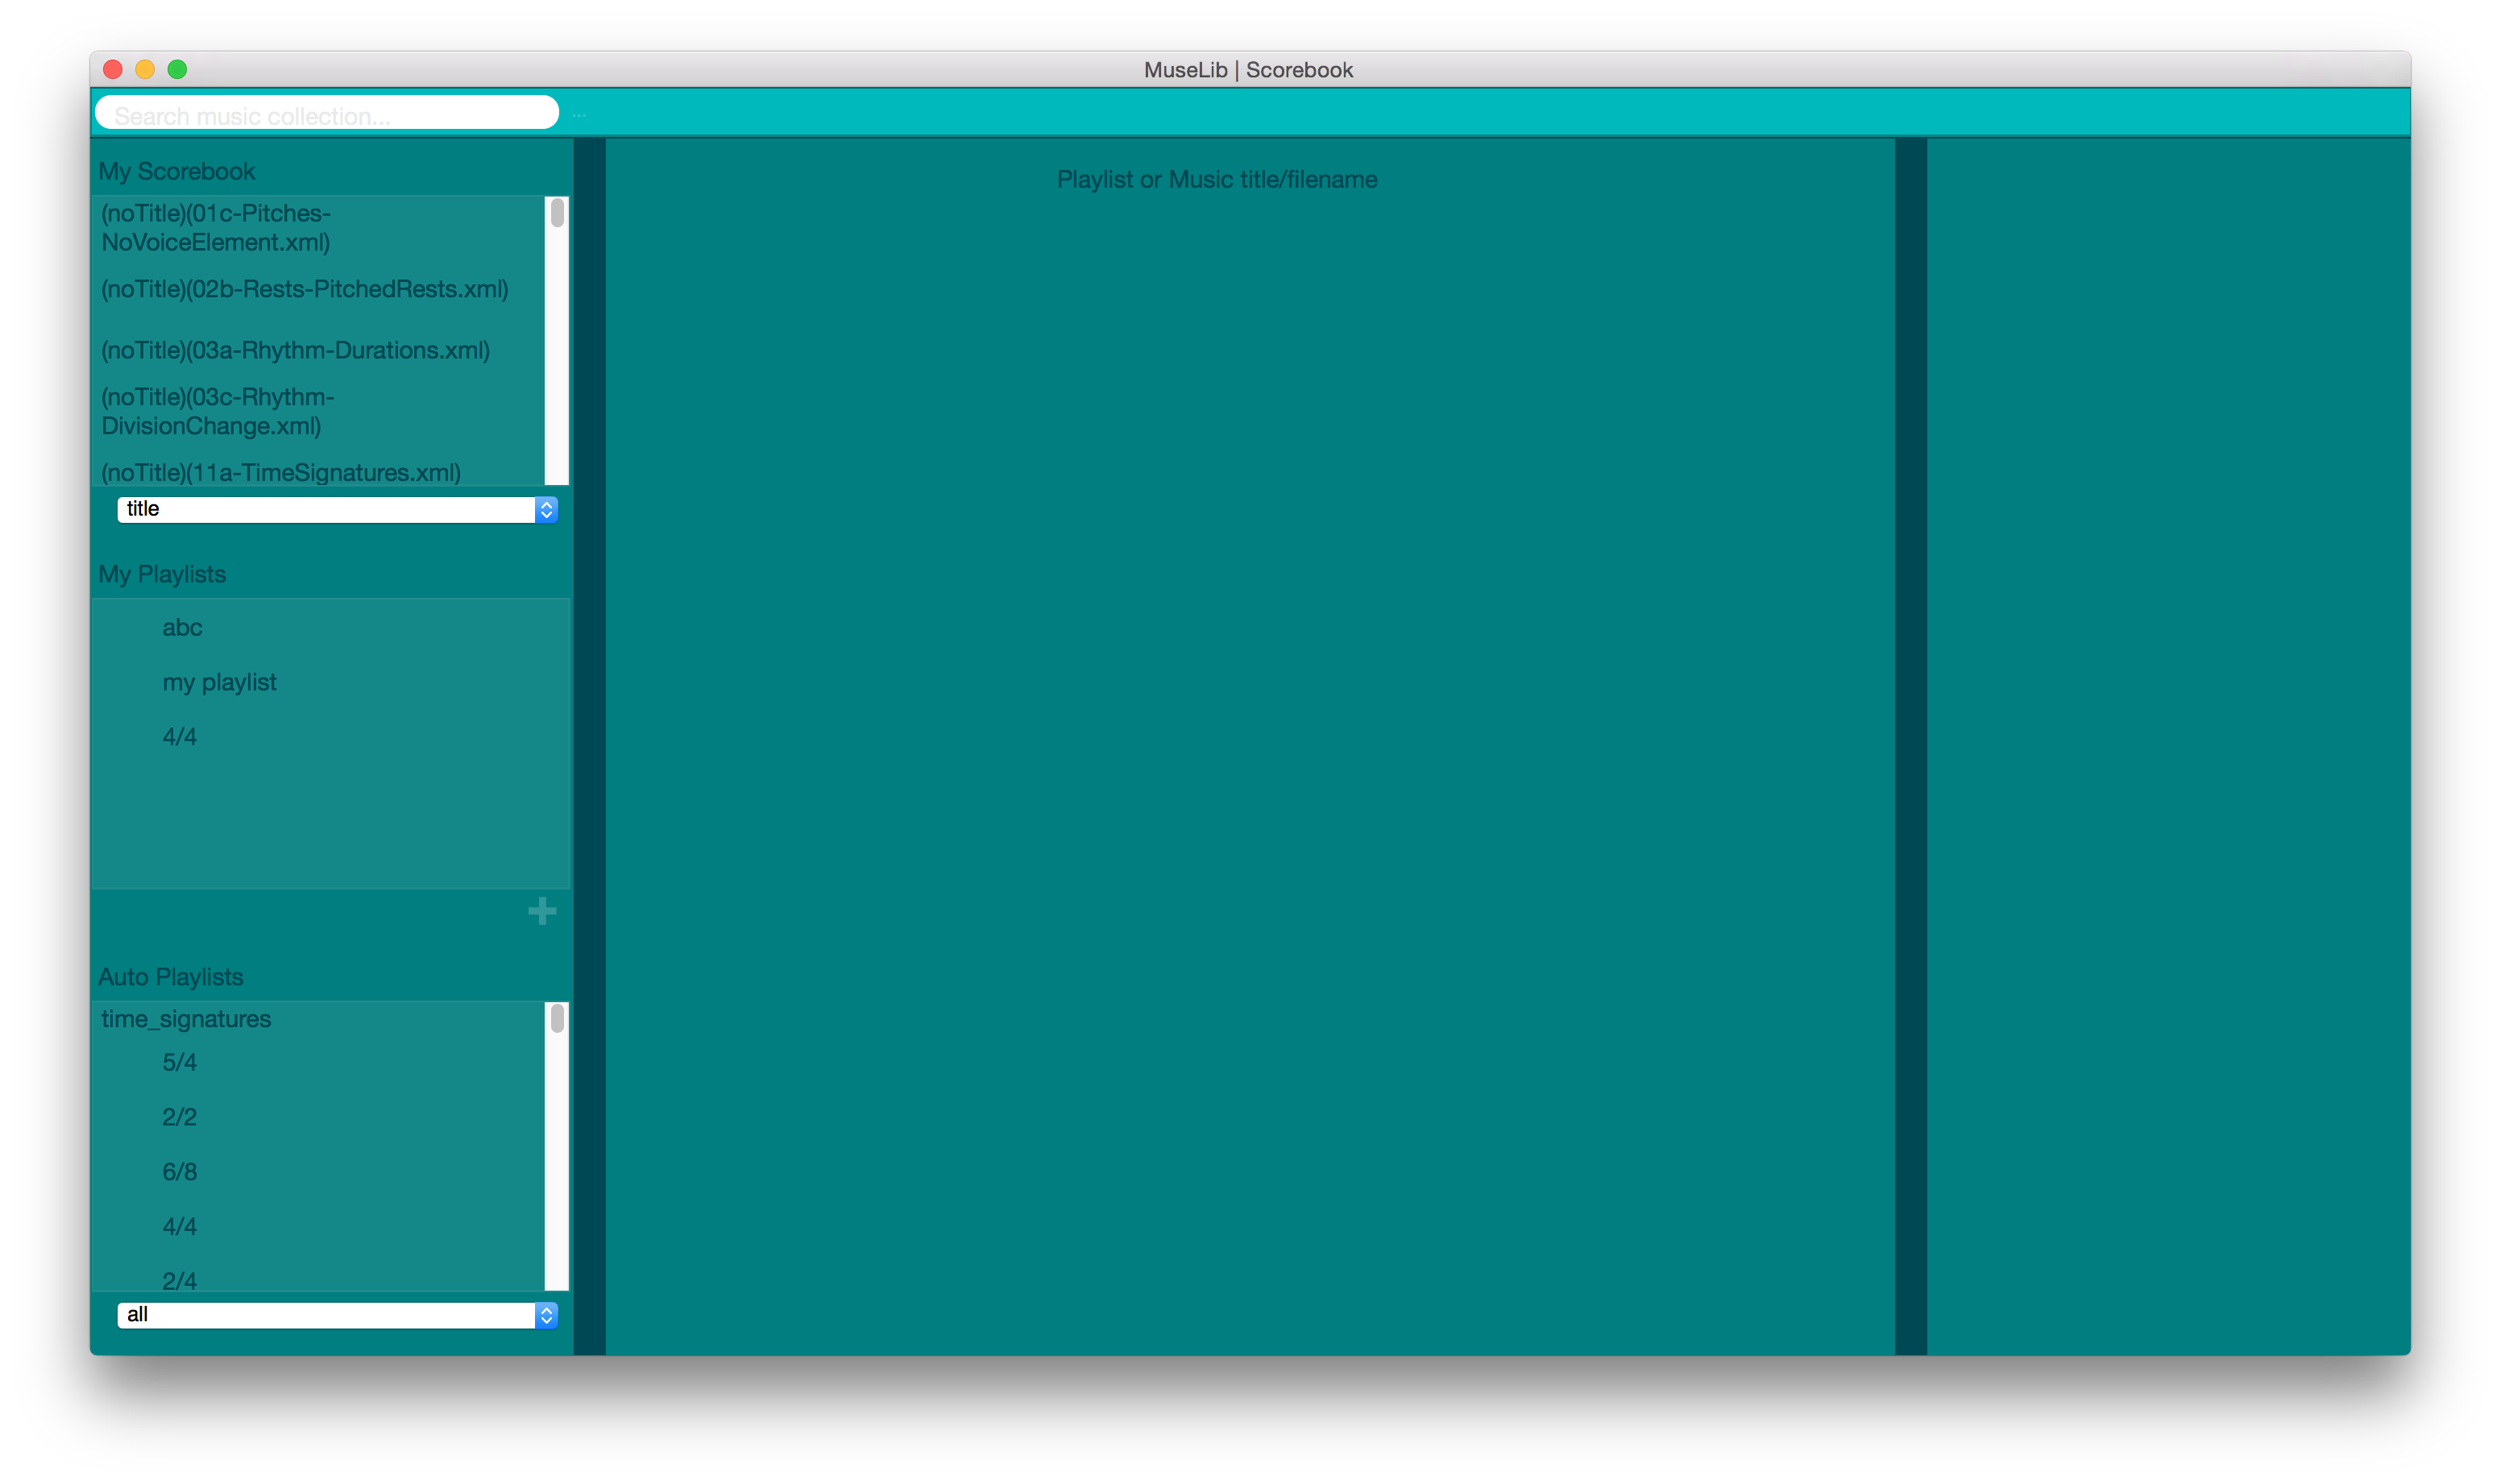
\includegraphics[width=400pt]{teal}
\caption{The teal theme}
\label{fig:theme4}	
\end{figure}

\subsection{Customising your widget views}
Any and all of the widgets to the right and left of the main pane can be hidden or displayed using the View menu, as shown in figure \ref{fig:view}.

\begin{figure}[H]
\centering
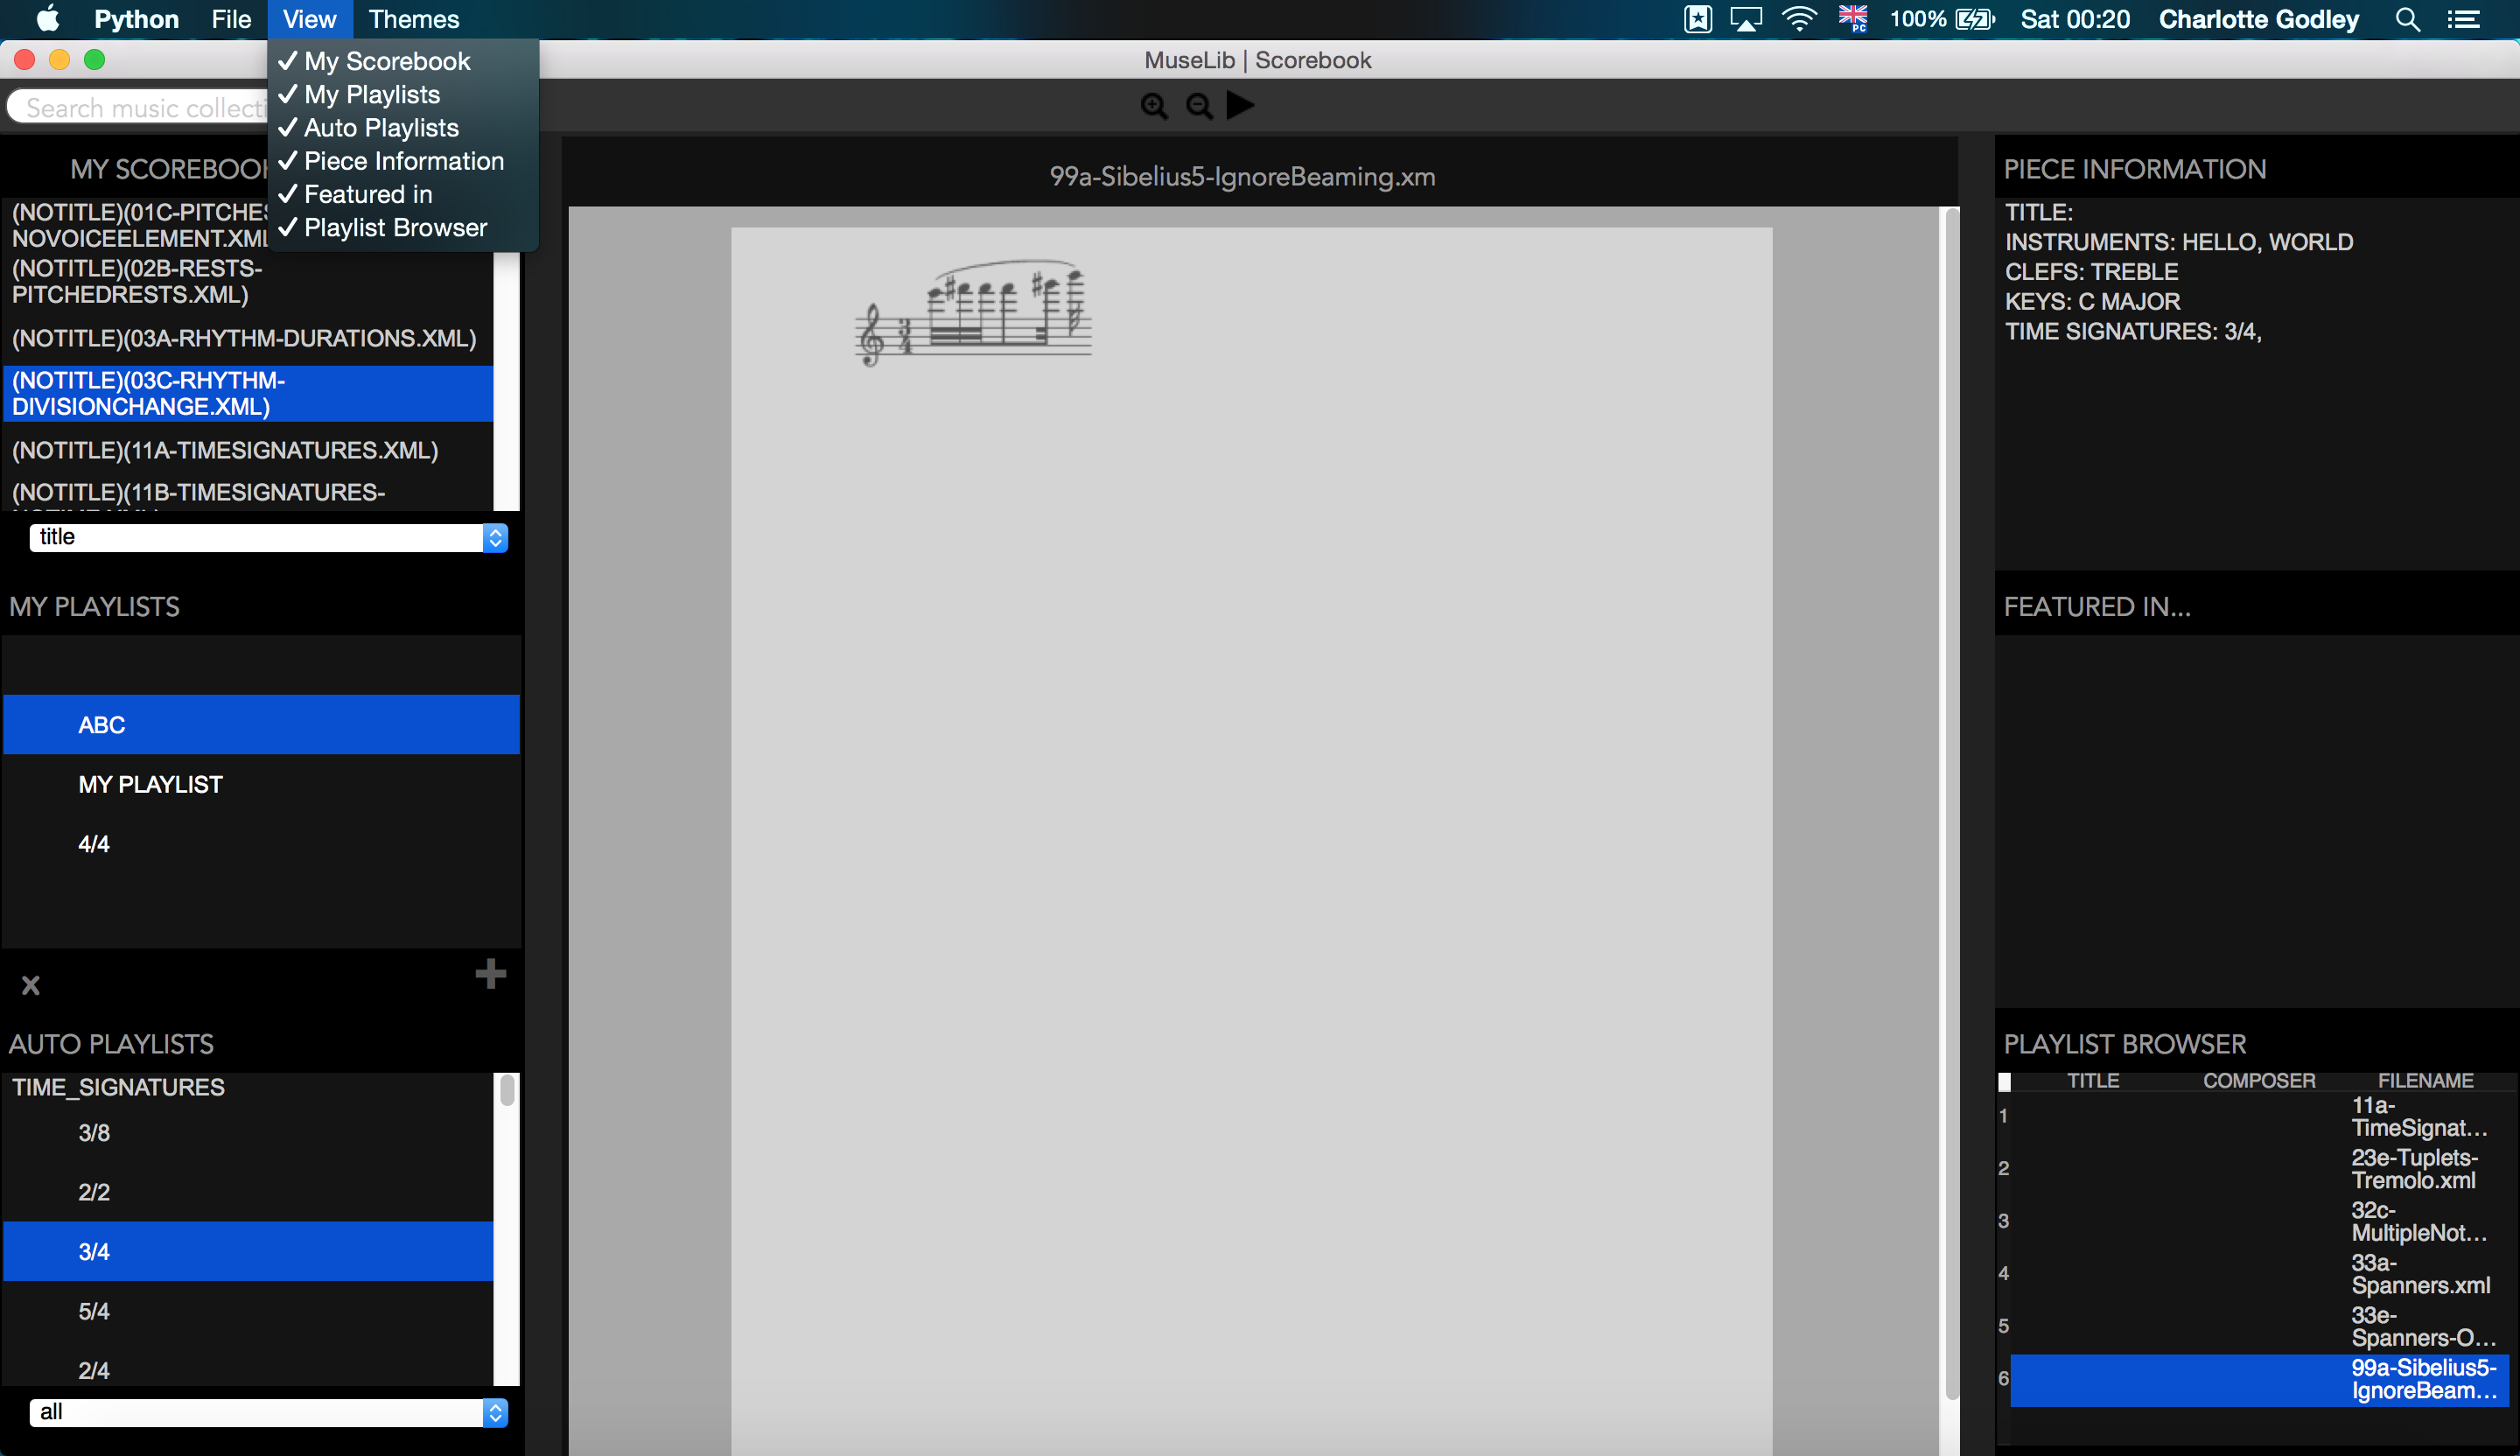
\includegraphics[width=500pt]{view}
\caption{The view menu}
\label{fig:view}	
\end{figure}


